\section{Markov Decision Process (MDP)}

\definecolor{darkgreen}{rgb}{0,0.6,0}

\begin{frame} 
\mode<presentation>{
    \begin{center} \huge
        \secname
    \end{center}
}
    \begin{center}
    A formalized description of the \underline{environment} in RL\footnote{Recommended reading 
\citep{sutton1998introduction} also video lectures by David Silver}
    \end{center}
\end{frame}


\begin{frame}\frametitle{\secname}
    
\begin{block}{Assumption of MDP}
The environment is fully observable. There is a complete characterization of what's going on and where everything is.
\end{block}

The other case would be \emph{partially observable} MDP (POMDP)

\end{frame}


\begin{frame}\frametitle{\secname}

\begin{block}{What do we want to do}
Maximize, not just immediate rewards but the \emph{cumulative sum of rewards} or ``return''.
\slidesonly{\vspace{-3mm}}
\begin{equation}
\mathit{return}(t) := \sum_{k=0}^{\infty} \gamma^k r(\vec x^{(t+k+1)}, \vec a^{(t+k+1)}) = \sum_{k=0}^{\infty} \gamma^k r^{(t+k+1)},
\end{equation}

where $\gamma \in \lbrack0,1)$ is referred to as the \emph{discount factor}.
 
\end{block}

\only<1>{
About the \emph{discount factor} $\gamma$:
}

\begin{itemize}
\only<1>{
\item It is possible for $\gamma$ to be $=1$.\\

\question{Under what condition can $\gamma$ be $=1$}\\


\mode<article>{
- $\gamma$ can be $=1$ if the length of the sequence is guaranteed to be finite.
}
}

\pause

\item \question{What does $\gamma \rightarrow 0$ imply?}\\

- preference for short term rewards

\pause

\item \question{What does $\gamma \rightarrow 1$ imply?}\\

\pause

- emphasis on long-term returns, indifference to delay.

\end{itemize}

\end{frame}

\begin{frame}\frametitle{The discount factor}
 
\mode<presentation>{
\begin{equation}
\mathit{return}(t) := \sum_{k=0}^{\infty} \gamma^k r^{(t+k+1)},\quad \text{where }\gamma \in \lbrack0,1)
\end{equation}

}

\mode<article>{
\figref{fig:discount} illustrates how the choice of $\gamma$ controls how fast the discount factors decay over time.
}

\begin{center}
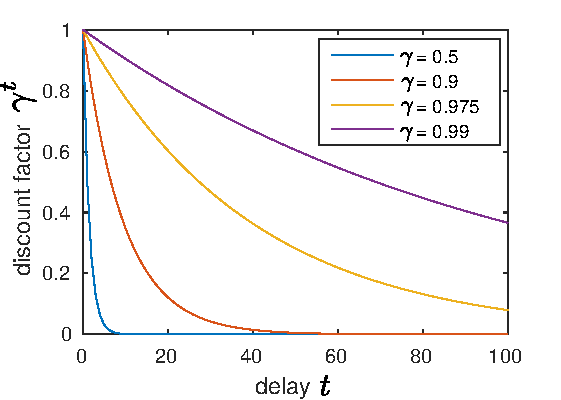
\includegraphics[width=6cm]{img/delay_discount}
\captionof{figure}{modulating returns with different discount factors}
\label{fig:discount}
\end{center}

\slidesonly{\vspace{-3mm}}
\slidesonly{\textbf{(see blackboard)}}

\end{frame}

\begin{frame}

\question{Why do we discount future rewards? What criteria goes into choosing $\gamma$?}\\

\pause

\begin{itemize}
\item Uncertainty of the future
\item Imperfections in the model (we don't trust its decisions completely)
\item mathematically convenient, the sum does not explode
\item avoids $\infty$ returns due to possible cycles in our MDP
\item behavioral arguments (animals and humans seem to apply a similar discounting)\\
``A bird in the hand is worth two in the bush''
\item financially realistic (accounts for inflation)
\end{itemize}

\end{frame} 

\subsection{The value function}


\definecolor{darkgreen}{rgb}{0,.5,0}
\definecolor{discount}{rgb}{.75,0,.75}
\definecolor{expect}{rgb}{0,.5,.5}
\definecolor{chain}{rgb}{.75,.5,0}

\begin{frame}\frametitle{\subsecname}

The (state) value function $\corresponds$ the expected sum of discounted future rewards

\question{What does the value function represent?}

\begin{itemize}
\item The long-term value of some state $\vec x$,
\item the expected return from starting in $\vec x^{(0)}$,
\item we have a preference for high expectations and MDPs maximize this quantity
\end{itemize}

\end{frame}

\begin{frame}\frametitle{\subsecname}

\mode<presentation>{
The value function $\corresponds$ the expected sum of discounted future rewards
}

For a fixed policy ${\color{policy}\pi}$:

	\only<1-4>{
	
	\begin{itemize}
		\item a \textbf{value function} measures the quality 
			of a policy $\pi$ in state $\vec x^{(0)}$
			\iitem{$V^\pi(\vec x^{(0)})$ is
				the {\em \visible<1->{{\color{expect}expected}} 
				\visible<2->{{\color{chain}{%
						\only<3>{\color{discount}}%
						\visible<3->{infinite} 
					}sum} of}
				\visible<3->{{\color{discount} discounted}} 
				\visible<2->{future}
				\visible<1->{{\color{reward}reward\visible<2->{s}}}}}
	\end{itemize}
	\only<1,3>{\vspace{1mm}}
	
	\begin{equation}
				V^\pi(\vec x^{(0)}) 
				\;\;=\;\; \visible<1->{{ \color{expect}	\E\bigg\lbrack }} 
					\visible<2->{{\color{chain}\sum_{t=0}^{
						\slidesonly{\only<2>{H}}%
						\only<3->{{\color{discount}\infty}}}}}
				\visible<3->{{\color{discount} \gamma^t} \,}
				{\color{reward} r(
					\slidesonly{\only<1>{{\color{black} \vec x^{(0)}}}}
					\only<2->{{\color{trans} \vec x^{(t)}}}, 
					{\color{policy}\vec a^{(\slidesonly{\only<1>{0}}\only<2->{t})}}
				) } 
				{ \color{expect}
					\,\bigg| \begin{array}{c}
							\scriptstyle {\color{policy}
								\vec a^{(\slidesonly{\only<1>{0}}\only<2->{t})} 
								\;\sim\; \pi(\cdot\,|\,
									\vec x^{(\slidesonly{\only<1>{0}}\only<2->{t})}) 
								}\;\;\;\\
							\visible<2->{{\color{trans}
								\scriptstyle \vec x^{(t+1)} \;\sim\; 
								P(\cdot \,|\, \vec x^{(t)}, \vec a^{(t)})
							}}
					\end{array}\kern-1ex 
					\bigg\rbrack
				} 
				\visible<3->{\,,\quad {\color{discount}\gamma \in \lbrack0, 1)} \,.}
	\end{equation}
	}
    \only<5>{
    \mode<presentation>{
    \begin{center}
		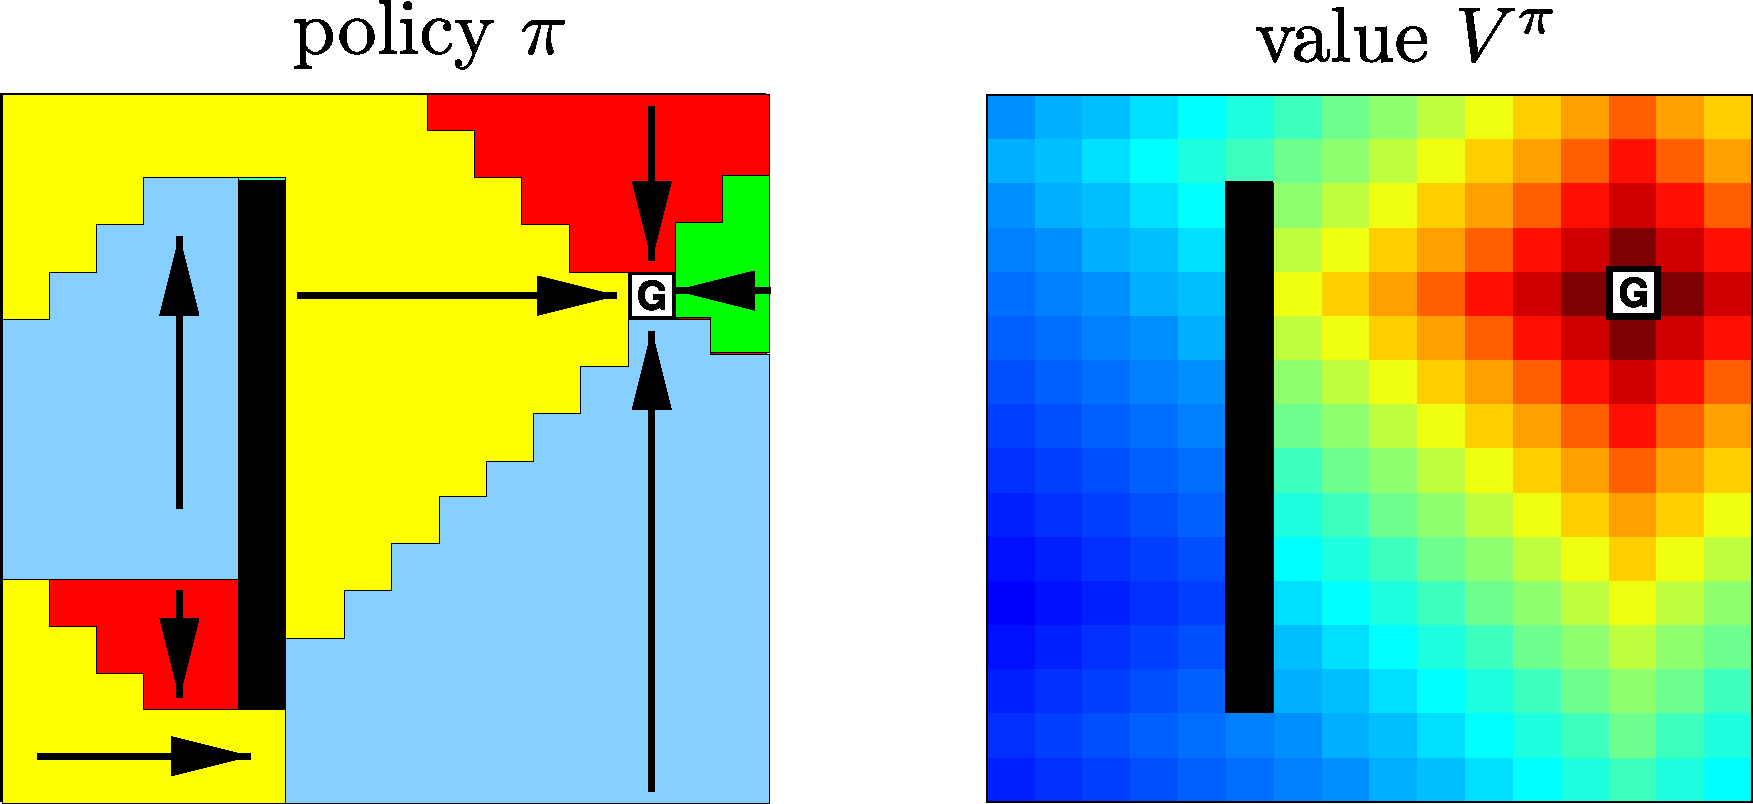
\includegraphics[trim={15cm 0 0 0mm},clip, height=3.cm]{img/nav_policy_and_value}
	\end{center}
    }
    }
    
    \visible<4,5>{
    
    
	In other textbooks you may find:
	
	\begin{align}
	V^\pi(\vec x_i) = \kern-1ex \overbrace{V^\pi_i}^{\text{shorthand}} \kern-1ex = 
	\E \bigg\lbrack
	\sum_{t=0}^{\infty} \gamma^t r(\vec x^{(t)}, \vec a^{(t)}) \;\Big|\; \vec x^{(0)} := \vec x_i
	\bigg\rbrack\,, \; i=1,\ldots,S
	\end{align}
	
	$\E\lbrack\cdot\rbrack$ is w.r.t $\{\vec x^{(t)}, \vec a^{(t)}\}$

    }

\end{frame}
